Norint atlikti filtravimo operaciją, reikalingas tam tikras modelis, kuriuo pagalba bus atliekama pati operacija.
Modelis apibūdina nagrinėjamą sistemą, kokios komponentės, kaip priklauso nuo esamų parametrų.
Visas žinias apie sistemą turi pateikti modelį kurianti pusė.

\subsection{Pradinis modelis}

Naudojamas jutiklis yra pagreičio jutiklis.
Pagreičio jutiklis grąžina momentinį pagreičio pokytį duotuoju matavimo gavimo metu, $a(t)$.
Tokių duomenų realus pavyzdys pateikiamas \ref{fig:ax_accel} pav.

Turėdami pagreičio duomenis, laiko momentu galima gauti greičio duomenis $v(t)$, \ref{fig:ax_velocity} pav.

\begin{equation}
    v(t) = \int_0^t a(t) \delta t
\end{equation}

Pozicijos pokytis $s(t)$ priklauso nuo objekto greičio $v(t)$, \ref{fix:ax_distance} pav.

\begin{equation}
    s(t) = \int_0^tv(t) \delta t
\end{equation}

Iš to seka, kad norint gauti sistemos poziciją, pagreitį reikia integruoti du kartus, \ref{fig:ax_accel_velocity_distance} pav.

\begin{equation}
    s(t) = \int_0^tv(t) \delta t = \int_0^t \int_0^t a(t) \delta t \delta t
\end{equation}

\begin{figure}
    \centering
    \subfloat[
        Vienos ašies pagreičio jutiklio matavimo duomenys
    ]{
        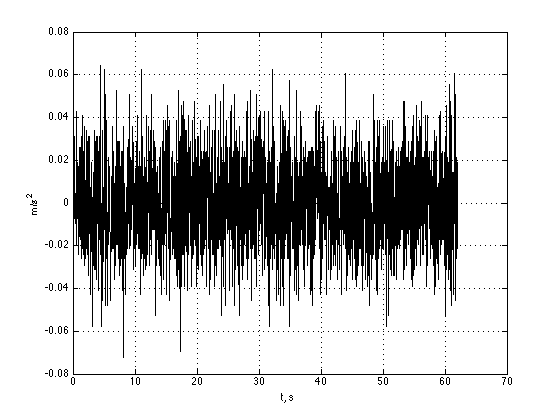
\includegraphics[
            width=0.4\textwidth
        ]{img/ax_accel.png}
        \label{fig:ax_accel}
    }
    \qquad
    \subfloat[
        Greičio duomenys, gauti integruojant pagreičio jutiklio vienos ašies duomenis
    ]{
        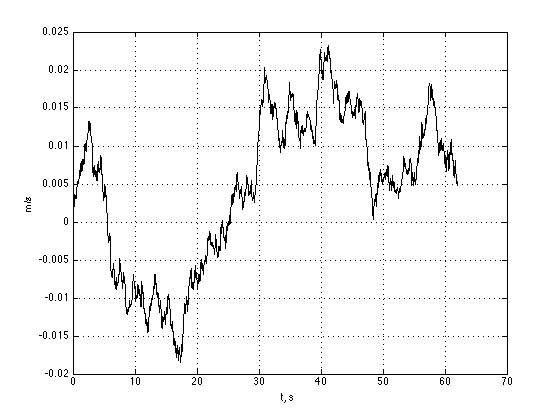
\includegraphics[
            width=0.4\textwidth
        ]{img/ax_velocity.png}
        \label{fig:ax_velocity}
    }
    \qquad
    \subfloat[
        Atstumo duomenys, gauti integruojant greičio duomenis pagal \ref{fig:ax_velocity}
    ]{
        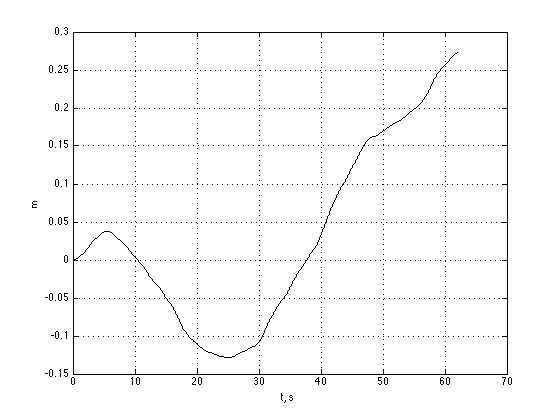
\includegraphics[
            width=0.4\textwidth
        ]{img/ax_distance.png}
        \label{fix:ax_distance}
    }
    \caption{Atstumo duomenis, gaunami iš pagreičio jutiklio vienos ašies duomenų}
    \label{fig:ax_accel_velocity_distance}
\end{figure}


Tokiu būdu gaunamas paprasčiausias matematinis modelis, kurio pagalba galima nustatyti dabartinę objekto poziciją.
Didžiausias šito modelio trūkumas, kuris matosi ir pateiktuose \ref{fig:ax_accel_velocity_distance} pavyzdžiuose, yra triukšmo dauginimas dėl dvigubo integravimo.
Pagreitis turi labai didelį matavimo triukšmą.
Integruojant vieną kartą, triukšmo įtaka matavimui yra padidinama du kartus.
Integruojant du kartus -- triukšmas padidėja keturis kartus.

\subsection{Kalman filtro modelis}

Kalman filtras reikalauja modelį aprašyti priklausomybės lygčių sistema.
Sistema turi apibūdinti gaunamų duomenų priklausomybę nuo galutinės sistemos būsenos.
Aprašymas pradedamas nuo pagreičio matavimo matmens

\begin{equation}
    a(t) = a(t)
\end{equation}

Greitis priklauso nuo greičio, kuris buvo vienu laiko momentu prieš, ir nauju pagreičiu

\begin{equation}
    v(t) = v(t-1) + a(t) * \delta t
\end{equation}

Pozicija priklauso nuo prieš tai buvusios pozicijos, dabartinio greičio poslinkio, bei pagreičio kvadrato

\begin{equation}
    s(t) = s(t-1) + v(t-1) + \frac{a(t)}{2}\delta t^2
\end{equation}

Iš šitų lygčių yra sudaromas sistemos būsenos modelis

\begin{equation}
    \hat{x} = \begin{cases}
        s(t-1) + v(t-1) + \frac{a(t)}{2}\delta t^2 \\
        v(t-1) + a(t) * \delta t \\
        a(t)
    \end{cases}
\end{equation}

Kadangi iš viso mes turime tris ašis, modelis patrigubėja ir iš viso jį sudaro

\begin{equation}
    \hat{x} = [ x, y, z, \dot{x}, \dot{y}, \dot{z}, \ddot{x}, \ddot{y}, \ddot{z}]^T,
\end{equation}
kur $\dot{x}$ yra pozicijos pirmą išvestinė -- greitis, $\ddot{x}$ yra pozicijos antra išvestinė -- pagreitis.

Galutinė sistemos būsenos matrica atrodo

\begin{equation}
    F = \begin{bmatrix}
        1 & 0 & 0 & dT & 0 & 0 & 0.5*dT^2 & 0 & 0 \\
        0 & 1 & 0 & 0 & dT & 0 & 0 & 0.5*dT^2 & 0 \\
        0 & 0 & 1 & 0 & 0 & dT & 0 & 0 & 0.5*dT^2 \\
        0 & 0 & 0 & 1 & 0 & 0 & -dT & 0 & 0 \\
        0 & 0 & 0 & 0 & 1 & 0 & 0 & -dT & 0 \\
        0 & 0 & 0 & 0 & 0 & 1 & 0 & 0 & -dT \\
        0 & 0 & 0 & 0 & 0 & 0 & 1 & 0 & 0 \\
        0 & 0 & 0 & 0 & 0 & 0 & 0 & 1 & 0 \\
        0 & 0 & 0 & 0 & 0 & 0 & 0 & 0 & 1
    \end{bmatrix},
\end{equation}
kur $dT$ yra laikas, nusakantis kaip dažnai buvo daromi matavimai.

Kalman filtro veikimui yra reikalauja turėti matavimų matricą.
Matavimų matrica nurodo, kuris iš modelio komponentų yra pats matavimas.
Šiuo atveju egzistuoja trys pagreičio komponentės, kurios nusako atliekamus matavimus.

\begin{equation}
    H = \begin{bmatrix}
        1 & 0 & 0 & 0 & 0 & 0 & 0 & 0 & 0 \\
        0 & 1 & 0 & 0 & 0 & 0 & 0 & 0 & 0 \\
        0 & 0 & 1 & 0 & 0 & 0 & 0 & 0 & 0
    \end{bmatrix}
\end{equation}

Pasirinkus matavimo matrica, toliau reikia pasirinkti dvi triukšmo įverčius.
Pirmas įvertis $q$, kuris nusako Kalman filtro darbo proceso triukšmą.
Antras įvertis $r$ yra matavimo triukšmas. 
Matavimo triukšmo įvertį galima nustatyti dviem keliais. 
Pirmas kelias yra eksperimentinis -- atlikti stabilios matavimus ant stabilios platformos ir panaudoti gautą nuokrypį kaip matavimo triukšmą.
Kitas kelias yra pasikliauti gamintojo nurodytu matavimo skaičiumi.
Proceso triukšmas modelyje šiuo atveju yra pasirenkamas lygus matavimo triukšmui modelio paprastumui ir jie abu yra lygus $0.1$.

Turint modelio lygčių sistemą, matavimo matricą bei triukšmus, galima pradėti dirbi su Kalman filtru.
Norint teisingai įvertinti Kalman filtro darbą su duomenimis, visi įėjimo duomenys yra modeliuojami paprastu $sin$ signalu, pridedant atsitiktinį baltą triukšmą.
Signalo pavyzdys pateikiamas \ref{fig:sin_acc_data_with_noise} pav.
Kaip matosi iš grafiko, signalas pats turi labai daug triukšmo, tačiau seka labai specifinį kelią, kurį galima atsekti su paprastu vidurkinimu.
Toks signalas nėra pilnai atsitiktinis, jis turi kažkokį dėsnį.
Atlikus dvigubą originalaus signalo integravimą, gaunamas atstumo pokytis \ref{fig:sin_distance_data_with_noise} pav.
Tiesinį Kalman filtro modelio rezultatas bus lyginamas su šiuo rezultatu ir bus laikomas teisingo rezultato etalonas.

\begin{figure}
    \centering
    \subfloat[Palyginimui naudojamas $sin$ signalas, su pridėtu baltu triukšmu]{
        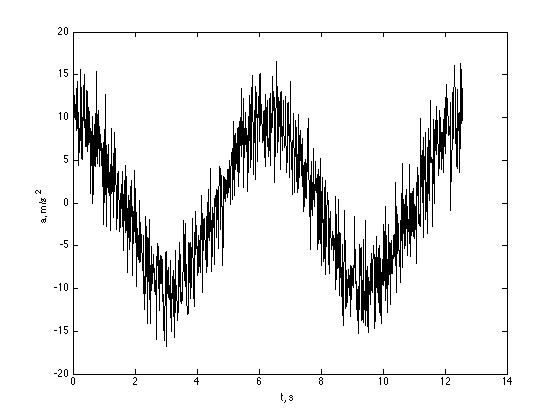
\includegraphics[
            width=0.45\textwidth
        ]{img/sin_acc_data.png}
        \label{fig:sin_acc_data_with_noise}
    }
    \qquad
    \subfloat[Atstumo pokytis, dvigubai integruojant $sin$ signalą]{
        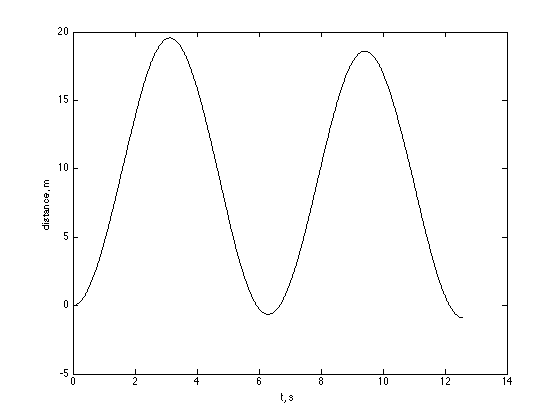
\includegraphics[
            width=0.45\textwidth
        ]{img/sin_acc_distance_data.png}
        \label{fig:sin_distance_data_with_noise}
    }    
\end{figure}

Pateikus į tiesinį Kalman filtrą duomenis, kuris remiasi ankščiau aprašytomis lygtimis, gaunamas rezultatas, kuris yra pateikiamas \ref{fig:linear_kalman_filter_sin} pav.
Duotas grafikas pateikia esminį tiesinio Kalman filtro naudojimo trūkumą duotos problemos atveju.
Esami duomenys visiškai neturi jokio tiesinės interpretacijos, todėl tiesinis Kalman filtras šiuo atveju nėra tinkamas.
Reikia panaudoti tokį sprendimą, kurį galima būtų pritaikyti ne tiesinėms sistemoms.

\begin{figure}
    \centering
    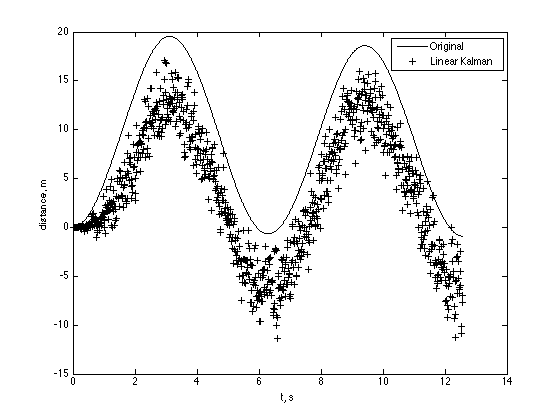
\includegraphics[
        width=0.6\textwidth
    ]{img/linear_kalman_filter.png}
    \caption{Tiesinio Kalman filtro pozicijos pokyčio rezultatas, lyginant su pradiniais duomenimis}
    \label{fig:linear_kalman_filter_sin}
\end{figure}

\subsection{Išplėstas Kalman filtras}

Išplėstas Kalman filtras yra ne tiesinis Kalman filtras.
Tai yra pasiekiama, panaudojus \textit{Jacobian} matricą, kurios pagalba ne tiesinė lygtis yra ištiesinama viename taške.

Modelis, kuris yra pateikiamas išplėstam Kalman filtrui turi būti ne matricinės, o lygčių sistemos formos, kadangi bus atliekamas diferencialinis skaičiavimas.
Dėl šitos priežasties, nagrinėjamas modelis yra perrašomas į lygčių sistemą

\begin{equation}
    \hat{x} = \begin{cases}
        x_1 + x_2 + x_3 * 0.5 * dT^2 \\
        x_2 + x_3 * dT \\
        x_3
    \end{cases}
\end{equation}

Toliau reikia perrašyti matavimo gavimo matricą į lygtį.
Kadangi matavimas yra gaunamas tiesiogiai, tai ir pati lygtis yra tiesinė lygtis

\begin{equation}
    h(\hat{x}) = x_3;
\end{equation}

Sekantis žingsnis yra nustatyti triukšmus.
Norint palyginti išplėstą Kalman filtro modelį su tiesiniu Kalman filtro modeliu, pasirenkamos tokie patys triukšmų įverčiai.

Pateikus tokius pačius duomenis, kaip ir į tiesinį Kalman filtrą, išplėstinio Kalman filtro rezultatas yra pateikiamas \ref{fig:extended_kalman_filter_sin} pav.

\begin{figure}
    \centering
    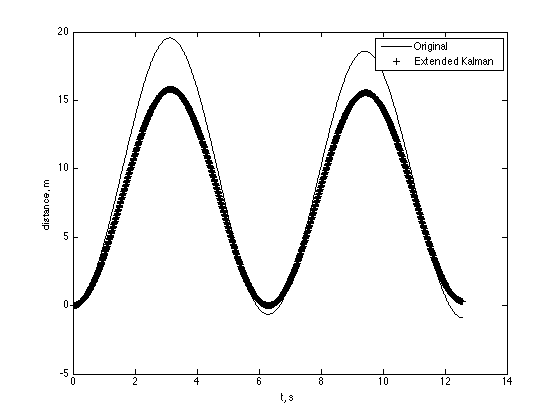
\includegraphics[
        width=0.6\textwidth
    ]{img/extended_kalman_filter.png}
    \caption{Išplėsto Kalman filtro pozicijos pokyčio rezultatas, lyginant su pradiniais duomenimis}
    \label{fig:extended_kalman_filter_sin}
\end{figure}

Lyginant tiesinio Kalman filtro \ref{fig:linear_kalman_filter_sin} rezultato ir išplėsto Kalman filtro rezultato \ref{fig:extended_kalman_filter_sin} grafikus, galima teigti, jog išplėstas Kalman filtras veikia geriau.
Tai yra logiškas ir lauktas rezultatas, kadangi išplėstas Kalman filtras yra skirtas dirbti su ne tiesinėmis sistemomis \cite{6851407}.
Šiuo atveju, uždaviniui spręsti galima pasirinkti išplėstą Kalman filtrą, tačiau tai yra ne paskutinis galimas problemos sprendimo būdas.
Šiuo metu labai pradeda populiarėti sekamas Kalman filtras, kuris sprendžia vieną pagrindinių išplėstinio Kalman filtro problemų -- tiesinimo triukšmą.

\subsection{Sekamas Kalman filtras}

Sekamas Kalman filtro modelio reikalavimai yra lygiai tokie patys, kaip išplėsto Kalman filtro, todėl modelio perrašinėti nėra tikslo.
Triukšmo įverčiai yra paliekami tokie patys, kaip ir tiesinio bei išplėstinio filtro atvejais.
Modelio veikimo rezultatas yra pateikiamas \ref{fig:unscented_kalman_filter_sin} pav.

\begin{figure}
    \centering
    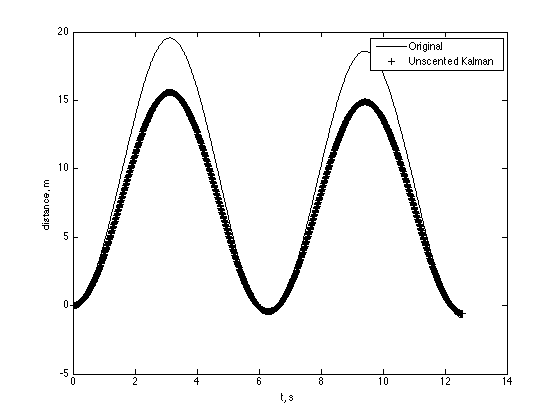
\includegraphics[
        width=0.6\textwidth
    ]{img/unscented_kalman_filter.png}
    \caption{Sekamo Kalman filtro pozicijos pokyčio rezultatas, lyginant su pradiniais duomenimis}
    \label{fig:unscented_kalman_filter_sin}
\end{figure}

\subsection{Modelio pasirinkimas}

Sekamas Kalman filtras \ref{fig:unscented_kalman_filter_sin}, lyginant su išplėstiniu Kalman filtru \ref{fig:extended_kalman_filter_sin} grafiškai neturi didelių privalumų.
Rezultato grafikas atrodo beveik identiškai.
Skirtumas matosi įverčiams artėjant prie nulinio pozicijos pokyčio, laiko momentu $t=6s$.
Išplėstas Kalman filtras toje srityje turi pokytį tarp realios reikšmės ir filtruotos reikšmės, tuo tarpu sekamas Kalman filtras priartėja prie realios reikšmės, ko pasekoje mažina klaidos vertę.

Norint išmatuoti skaitinėmis reikšmėmis šių trijų pateiktų filtrų tikslumų skirtumus, bus panaudota kryžminė koreliacija.
Kryžminė koreliacija yra plačiai naudojamas matas, nustatyti panašumus tarp dviejų signalų.
Kuo gautas skaitinis įvertis yra arčiau nulio -- tuo signalai yra panašesni.
Verta paminėti, kad šitas matavimas yra naudojamas metodų palyginimui.

\begin{table}
    \centering
    \caption{Kryžminės koreliacijos matavimo rezultatas kiekvienam filtrui}
    \label{table:kalman_filter_comparison}
    \begin{tabular}{|c|c|c|} \hline
        Filtras & Koreliacija \\ \hline
        Tiesinis Kalman filtras & 0.8811 \\ \hline
        Išplėstas Kalman filtras & 0.9989 \\ \hline
        Sekamas Kalman filtras & 1.0000 \\ \hline
    \end{tabular}
\end{table}

Pagal gautus duomenis, kurie yra pateikiami \ref{table:kalman_filter_comparison} lentelėje galima daryti išvadas, kad geriausiai duomenis filtruoja būtent Sekamas Kalman filtras ir netoli jo yra išplėstas Kalman filtras.
Remiantis šiuo rezultatu, filtro įgyvendinimui yra pasirenkamas Sekamas Kalman filtras.

